\section{Introduction}
\subsection{Basics}
\begin{frame}{Outline}
\tableofcontents[currentsection]
\end{frame}


\begin{frame}{Let's get on the same page}
 \begin{itemize}
  \item \large{We should know what a \textit{state} is} \pause
	\begin{itemize}  	
  	\item i.e. a psd matrix $\rho$ that satisfies Tr$(\rho)=1$ \pause 
	\end{itemize}
 \item \large{We should know what the \textit{tensor product} does} \pause
	\begin{itemize}
		   \item We use the Kronecker product  $A \otimes B = \begin{pmatrix}
a_{11}B & \dots & a_{1n}B \\
\vdots && \vdots \\
a_{n1}B & \dots & a_{nn}B
\end{pmatrix}$
	\end{itemize}  
   \item \large{We should be familiar with the \textit{Dirac notation}} \pause
	\begin{itemize}	 
  	\item $\vert \psi \rangle$ is a vector in $\mathbb{C}^n$ and $\langle \psi \vert$ is its conjugate transpose
 \end{itemize}
 \end{itemize}

\begin{block}{Quantum systems}
	\begin{itemize}
		\item A quantum system is a portion of the whole universe. For example a set electrons. 
		\item A quantum system $X$ is associated with a copy of $\mathbb{C}^k$ 
		\item It may consist of subsystems $X_1, \dots , X_N$ each of which is associated with a copy of $\mathbb{C}^{n_i}$. In this case $k = n_1 \dots n_N$
	\end{itemize}
\end{block}

\end{frame}

\begin{frame}{Measurements}
Physical quantities can be measured. But what is a measurement mathematically? \pause
\begin{itemize}
    \item A measurement can be performed on a system $X$ that is in state $\rho$ \pause
    \item We want the set of outcomes to finite. Let $\mathcal{A}$ be this set \pause
    \item The outcome of a measurement is supposed to be a random variable $\chi$ that takes values in $\mathcal{A}$ with a certain probability \pause
    \item This can be achieved:
\end{itemize}
\begin{definition}{Measurement}
\begin{itemize}    
     \item We define a measurement by a set of psd matrices $\{ F^a \}_{a\in \mathcal{A}} \subseteq \mathbb{C}^{n \times n}$ that sum up to the identity matrix, i.e. $\sum_{a \in \mathcal{A}} F^a = I$
    \item The outcome of a measurement is a random variable $\chi$ with probability distribution: $\mathbb{P}[ \chi = a ] = \text{Tr}(\rho F^a)$
     \item A projective measurement is defined by psd matrices that satisfy $F^aF^b = \delta_{ab}F^a \text{ } \forall a,b \in \mathcal{A}$
\end{itemize}
\end{definition}
\end{frame}    
    
\begin{frame}
\begin{itemize}   
    \item To define an expected value we define outcomes in $\mathcal{A}$ as real numbers \pause
    \item $\mathbb{E} [\chi ] \overset{def}{=} \sum_{a \in \mathcal{A}} a \text{Tr} ( \rho F^a ) \overset{lin}{=}  \text{Tr} ( \rho ( \sum_{a \in \mathcal{A}} a F^a))$ \pause
    \item $\sum_{a \in \mathcal{A}} aF^a$ is called observable \pause
    \item A simple case we will use later are $\{ -1, 1 \}$-valued observables \pause
    \item if we consider projective measurements we have
\end{itemize}
    \begin{equation*}
(F^+-F^-)^2 = \underbrace{F^{+^2}}_{= F^+}- \underbrace{F^+F^-}_{\delta_{+-}=0} + \underbrace{F^{-^2}}_{F^-} = F^+ + F^- = I
\end{equation*}
\begin{itemize}
    \item i.e. a $\{ -1, 1 \}$-valued observable is both unitary an Hermitian 
\end{itemize}

\end{frame}

\begin{frame}{Doling out subsystems}
\begin{itemize}
    \item Consider a system $X$ consisting of subsystems $X_1, \dots X_N$ which we distribute among $N$ parties, which may be located anywhere in the universe \pause
    \item The parties \textit{share} the state $X$ is in \pause
    \item Every party may perform a measurement on their subsystem $X_i$, i.e. there are $N$ sets of psd matrices $\{F^{a_1} \}_{a_1 \in \mathcal{A}_1} \in \mathbb{C}^{n_1 \times n_1}, \dots , \{F^{a_N} \}_{a_N \in \mathcal{A}_N} \in \mathbb{C}^{n_N \times n_N} $ \pause
\end{itemize}
    
\begin{block}{}
    The joint probability distribution of the $N$ measurement outcomes $\chi_1 , \dots , \chi_N$ is 
\begin{equation*}
\mathbb{P}\left[ \chi_1 = a_1, \chi_2 = a_2, \dots , \chi_N = a_N \right] = \text{Tr}(\rho F_1^{a_1} \otimes \dots \otimes F_N^{a_N}) 
\end{equation*}
\end{block}
\end{frame}

\begin{frame}{Entanglement}
\begin{itemize}
    \item We will only consider pure states meaning states that they have rank $1$ and therefore can be written as $\rho = \vert \psi \rangle \langle \psi \vert$
    \item A state is called product state if it can be written as $\vert \psi \rangle = \vert \psi_1 \rangle \vert \psi_2 \rangle \dots \vert \psi_N \rangle$
    \item When a vector $\vert \psi \rangle$ is referred to as a state we mean the matrix $\vert \psi \rangle \langle \psi \vert$
    \item A state that is not a product state is called entangled
\end{itemize}
    
\end{frame}

\begin{frame}{Example}
    \begin{itemize}
        \item Let $\vert \psi \rangle = \vert \psi_A \rangle \vert \psi_B \rangle$ be a system and give $\vert \psi_A \rangle$ to Alice and $\vert \psi_B \rangle$ to Bob
        \item Let them perform measurements $\{ G^b \}_{b \in \mathcal{B}}$ and $\{F^a \}_{a \in \mathcal{A}}$ on their respective quantum systems
        \item What is the  probability of Alice getting measurement outcome $\chi_A = a$ and Bob getting $\chi_B = b$?
    \end{itemize}
\end{frame}

\begin{frame}{Example}
\begin{flalign*}
\text{Tr}(\vert \psi \rangle \langle \psi \vert F^a \otimes G^b ) & = \langle \psi \vert F^a \otimes G^b \vert \psi \rangle \\
& = (\langle \psi_A \vert \otimes \langle \psi_B \vert) (F^a \otimes G^b )(\vert \psi_A \rangle  \otimes \vert \psi_B \rangle )\\
& = ((\langle \psi_A \vert F^a)\otimes (\langle \psi_B \vert  G^b))( \vert \psi_A \rangle \otimes \vert \psi_B \rangle) \\
& = \langle \psi_A \vert F^a \vert \psi_A \rangle \otimes  \langle \psi_B \vert G^b \vert \psi_B \rangle \\
&= \langle \psi_A \vert F^a \vert \psi_A \rangle  \langle \psi_B \vert G^b \vert \psi_B \rangle
\end{flalign*}
This is equal to the product of the probabilities of Alice measuring $a$ and Bob measuring $b$, i.e. the outcome do not correlate.
\end{frame}


\subsection{Nonlocal games}
\begin{frame}{Nonlocal games}
    \begin{itemize}
        \item Three participants: Alice, Bob and a referee
        \item Referee doles out a question $s$ to Alice and a question $t$ to Bob
        \item Alice and Bob are assumed to be located anywhere in the universe respectively 
        \item Alice and Bob must not communicate
        \item Alice sends answer $a$ Bob sends answer $b$ back to the referee, who then decides whether both win or both lose
    \end{itemize}
\end{frame}

\begin{frame}{Nonlocal games}
    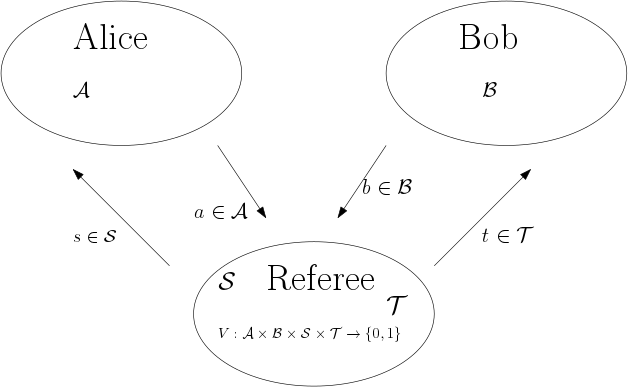
\includegraphics[scale=0.5]{Untitled.png}
\end{frame}

\begin{frame}{Mathematically speaking}
\begin{itemize}
    \item Four finite sets $\mathcal{A}, \mathcal{B}, \mathcal{S}, \mathcal{T}$
    \item probability distribution $\pi$ over $\mathcal{S} \times \mathcal{T}$ \\ $\pi : \mathcal{S} \times \mathcal{T} \rightarrow [0,1]$
    \item The referee sends with probability $\pi (s,t)$ $s$ to Alice and $t$ to Bob
    \item They answer with an element $a \in \mathcal{A}$ and $b \in \mathcal{B}$ respectively
    \item A map $V : \mathcal{S} \times \mathcal{T} \times \mathcal{A} \times \mathcal{B} \rightarrow \{ 0, 1 \}$
    \item They win if $V(s,t,a,b)=1$ and lose otherwise
\end{itemize}
\end{frame}

\begin{frame}{Classical strategies}
    \begin{itemize}
        \item All players know $\pi$ and $V$ and the information they received but not what the other players received
        \item They are allowed to agree on a strategy beforehand but must not communicate once the game started
        \item A deterministic strategy is a map $a : \mathcal{S} \rightarrow \mathcal{A}$ for Alice and $b : \mathcal{T} \rightarrow \mathcal{B}$ for Bob
        The winning probability then is:
    \end{itemize}
    \begin{equation*}
        \mathbb{E}_{s,t \sim \pi} \left[ V(a(s),b(t),s,t) \right]
\end{equation*}
\end{frame}

\begin{frame}{Quantum case}
\begin{itemize}
    \item Suppose Alice and Bob have a subsystem $X_A, X_B$ of a quantum system $X$ which is in state $\rho$, i.e. Alice and Bob share state $\rho$
    \item If the state is entangled measurements can give correlated measurement outcomes
    \item Alice and Bob may gain information by performing measurements
    \item Answering according to measurement outcomes could increase winning probability 
\end{itemize}
\end{frame}


\begin{frame}{Mathematically speaking}
\begin{itemize}
    \item A quantum system $X$ consisting of two $n$-dimensional subsystems $X_A, X_B$ in some entangled state $\rho$
    \item Alice performs a measurement $\{ F_s^a \}_{a\in \mathcal{A}}\subseteq \mathbb{C}^{n \times n}$ on her subsystem $X_A$ and Bob performs a measurement $\{ G_t^b\}_{b \in \mathcal{B}} \subseteq \mathbb{C}^{n \times n}$ on his subsystem $X_B$
    \item They send their measurement outcome as their answer to the referee
    \item Their winning probability is:
\end{itemize}
\begin{equation*}
\mathbb{E}_{s,t \sim \pi} \left[ \sum_{a \in \mathcal{A}} \sum_{b \in \mathcal{B}} \text{Tr}(\rho F_s^a \otimes G_t^b) V(a,b,s,t) \right]
\end{equation*}  
\end{frame}

\subsection{A special case of nonlocal games}
\begin{frame}{Two player XOR games}
\begin{itemize}
    \item Let the sets $\mathcal{A}$ and $\mathcal{B}$ be $\{0,1\}$, so Alice and Bob both answer either with $1$ or $0$
    \item The predicate $V$ is defined as $V(a,b,s,t) = [ a\oplus b = f(s,t)]$, where $f: \mathcal{S} \times \mathcal{T} \rightarrow \{0,1\}$
    \item A truth table for $a \oplus b$ looks like this
\end{itemize}
    \begin{center}
\begin{tabular}{l | c r }
$\oplus$ & 0 & 1 \\
\cline{1-3} 

0 & 0 & 1 \\
1 & 1 & 0 
\end{tabular}\\
\end{center}
\end{frame}

\begin{frame}{Bias and violation ratio}
\begin{itemize}
    \item Alice and Bob can always win with probability $\frac{1}{2}$ by flipping an unbiased coin
    \item The classical bias of an XOR game $G$ is defined as the difference of the probabilities of winning and losing for an optimal strategy and denoted by $\beta(G)$
    \item The bias $\beta^*(G)$of entangled strategies is calculated the same way 
    \item It is twice the amount by which the maximal winning probability exceeds $\frac{1}{2}$
    \item Since $\frac{1}{2}+ \gamma -(1-\frac{1}{2}-\gamma) = 2\gamma$
    \item The violation ratio is defined as $\frac{\beta^*(G)}{\beta(G)}$
\end{itemize}
    
\end{frame}

\begin{frame}{Signs and observables}
\begin{itemize}
    \item It is convenient to use the $\{-1,1\}$-basis instead of the $\{0,1\}$-basis for boolean valued objects.
    \item Let $a : \mathcal{S} \rightarrow \{ 0,1 \} \text{ and } b: \mathcal{T} \rightarrow \{ 0,1\}$ be classical strategies and $\pi$ the probability distribution the referee uses to pick $s,t$
    \item The bias is given by the probability under $\pi$ that $a(s) \oplus b(t) = f(s,t)$ minus the probability under $\pi$ that $a(s) \oplus b(t) \ne f(s,t)$
\end{itemize}
    
\end{frame}

\begin{frame}
This means the bias can be written as:
\begin{flalign*}
 \mathbb{E}_{(s,t) \sim \pi} \left[ (-1)^{[a(s) \oplus b(t) = f(s,t)]} \right] & = \\ = \mathbb{E}_{(s,t) \sim \pi} \left[ (-1)^{a(s) \oplus b(t) + f(s,t)} \right] =\\
 = \mathbb{E}_{(s,t) \sim \pi} \left[ (-1)^{a(s)}(-1)^{b(t)}(-1)^{f(s,t)} \right]
  \end{flalign*}    
And we can define the sign matrix $\Sigma_{s,t} = (-1)^{f(s,t)}$ and functions $\chi(s) = (-1)^{a(s)}$ and $\psi(t) = (-1)^{b(t)}$. So the bias is
\begin{equation*}
\mathbb{E}_{ ( s , t ) \sim \pi} \left[ \chi (s) \psi (t) \Sigma_{st} \right]
\end{equation*}
\end{frame}

\begin{frame}{}
\begin{itemize}
    \item The outcomes in an XOR game are $\{ 0,1 \}$
    \item Alice and Bob have measurements $\{ F_s^0, F_s^1 \}$ and $\{ G_t^0, G_t^1 \}$ and share an entangled state
    \item The probability of Alice and Bob answering with $a,b$ upon receiving $s,t$ respectively is $\langle \psi \vert F_s^a \otimes G_t^b \vert \psi \rangle$
    \item Lets calculate the expected value of $(-1)^{a \oplus b}$
\end{itemize}
\begin{flalign*}
(1)\cdot \mathbb{P}\left[ a = b \right] + (-1) \cdot \mathbb{P} \left[ a \ne b \right]  = \\ = \langle \psi \vert F_s^0 \otimes G_t^0 \vert \psi \rangle + \langle \psi \vert F_s^1 \otimes G_t^1 \vert \psi \rangle \\ - \langle \psi \vert F_s^1 \otimes G_t^0 \vert \psi \rangle - \langle \psi \vert F_s^0 \otimes G_t^1 \vert \psi \rangle \\
= \langle \psi \vert (F_s^0 - F_s^1) \otimes (G_t^0 - G_t^1) \vert \psi \rangle
\end{flalign*}
\end{frame}

\begin{frame}
\begin{itemize}
    \item Define $\{-1,1\}$-observables $F_s = F_s^0-F_s^1$ and $G_t=G_t^0-G_t^1$ with the property that its difference squared is the identity matrix
    \item Using this strategy the bias becomes
\end{itemize}
\begin{equation*}
\mathbb{E}_{(s,t) \sim \pi} \left[ \langle \psi \vert F_s \otimes G_t \vert \psi \rangle \Sigma_{s,t} \right]
\end{equation*}
\end{frame}

\begin{frame}{More generally speaking}
\begin{itemize}
    \item For any XOR game the bias is defined as the difference of the probabilities of winning and loosing \item Which is, if considering the $\{ -1, 1 \}$ basis, the expected value
    \item We are looking to maximize this quantity
\end{itemize}
    
\end{frame}

\begin{frame}{Classical strategies}
    When using classical strategies this is 
    \begin{flalign*}
\max \lbrace \mathbb{E}_{(s,t) \sim \pi} \left[ \Sigma_{st} \chi (s) \psi (t) \right] : \chi : \mathcal{S} \rightarrow \{ -1, 1 \}, \\ \psi : \mathcal{T} \rightarrow \{-1, 1 \} \rbrace
\end{flalign*} 

\end{frame}

\begin{frame}{Entangled strategies}
When using entangled strategies the winning probability might increase indefinitely with the dimensions, so we use the $\sup_{n \in \mathbb{N}}$
\begin{flalign*}
\sup_{n \in \mathbb{N}} \lbrace \mathbb{E}_{(s,t) \sim \pi} \left[ \Sigma_{st} \langle \psi \vert F_s \otimes G_t \vert \psi \rangle \right] : \vert \psi \rangle \in \mathbb{C}^{n} \otimes \mathbb{C}^{n} ,\\ F_s, G_t \in O(\mathbb{C}^n) \rbrace
\end{flalign*}
    
\end{frame}

\subsection{A specific example}
\begin{frame}{The CHSH game}
\begin{itemize}
    \item The CHSH game (Clauser, Horner, Shimony, Holt) is a two player XOR game with $\mathcal{A} = \mathcal{B} = \mathcal{S} = \mathcal{T} = \{0,1\}$ and $\pi$ being the uniform distribution
    \item  $f(s,t)= s \land t$, i.e. $f(1,1)=1$ and $f(0,0)=f(0,1)=f(1,0)=0$
    \item Alice and Bob can win $\frac{3}{4}$ of the games by using deterministic strategies $(0,0), (1,0) \text{ or } (0,1)$
\end{itemize}
\end{frame}

\begin{frame}{Quantum strategy}
\begin{itemize}
    \item Let Alice and Bob share an EPR state
    \item Define 
\end{itemize}
    \begin{equation*}
X = \begin{bmatrix}
0 & 1 \\
1 & 0
\end{bmatrix} , Y = \begin{bmatrix}
0 & -i \\ 
i & 0 
\end{bmatrix}
\end{equation*}
\begin{itemize}
    \item $XY +YX = 0$ and $X^2=Y^2=I$
    \item For Alice define the observable for question $0$ by $F_0=X$ and for question $1$ by $F_1=Y$
    \item Bobs observables are going to be $G_0 = (X-Y)/ \sqrt{2}$ for question $0$ and $G_1 = (X+Y)/\sqrt{2}$ for question $1$
\end{itemize}
\end{frame}

\begin{frame}{}
    The following auxiliary calculations will be helpful later: 
\begin{flalign*}
\langle \text{EPR} \vert X \otimes X \vert \text{EPR} \rangle & = \frac{1}{2} \begin{pmatrix}
1 & 0 & 0 &1
\end{pmatrix} \begin{pmatrix}
0 & 0 & 0 & 1 \\
0 & 0 & 1 & 0 \\
0& 1 & 0 & 0 \\
1 & 0 & 0 & 0
\end{pmatrix} \begin{pmatrix}
1 \\ 0 \\ 0 \\ 1
\end{pmatrix}\\
& = \frac{1}{2} \begin{pmatrix}
1 &0&0&1
\end{pmatrix} \begin{pmatrix}
1 \\ 0 \\ 0 \\1
\end{pmatrix} = \frac{2}{2} = 1\\
\end{flalign*}
\end{frame}

\begin{frame}{}
    \begin{flalign*}
\langle \text{EPR} \vert Y \otimes Y \vert \text{EPR} \rangle & = \frac{1}{2} \begin{pmatrix}
1 & 0 & 0 &1
\end{pmatrix} \begin{pmatrix}
0 & 0 & 0 & -1 \\
0 & 0 & 1 & 0 \\
0& 1 & 0 & 0 \\
-1 & 0 & 0 & 0
\end{pmatrix} \begin{pmatrix}
1 \\ 0 \\ 0 \\ 1
\end{pmatrix}\\
& = \frac{1}{2} \begin{pmatrix}
-1 &0&0&-1
\end{pmatrix} \begin{pmatrix}
1 \\ 0 \\ 0 \\1
\end{pmatrix} = -1\\
\end{flalign*}

\end{frame}

\begin{frame}{}
\begin{flalign*}
\langle \text{EPR} \vert X \otimes Y \vert \text{EPR} \rangle & = \frac{1}{2} \begin{pmatrix}
1 & 0 & 0 &1
\end{pmatrix} \begin{pmatrix}
0 & 0 & 0 & -i \\
0 & 0 & i & 0 \\
0& -i & 0 & 0 \\
i & 0 & 0 & 0
\end{pmatrix} \begin{pmatrix}
1 \\ 0 \\ 0 \\ 1
\end{pmatrix}\\
& = \frac{1}{2} \begin{pmatrix}
i &0&0&-i
\end{pmatrix} \begin{pmatrix}
1 \\ 0 \\ 0 \\1
\end{pmatrix} = 0\\
\langle \text{EPR} \vert Y \otimes X \vert \text{EPR} \rangle & = 0
\end{flalign*}
\end{frame}

\begin{frame}{}
    Lets calculate the expected values of the sign $a \oplus b$: 
\begin{flalign*}
   \langle \text{EPR} \vert F_0 \otimes G_0 \vert \text{EPR} \rangle = \langle \text{EPR} \vert X \otimes \frac{1}{\sqrt{2}}(X-Y) \vert \text{EPR} \rangle  \\
= \langle \text{EPR} \vert X \otimes \frac{1}{\sqrt{2}}X \vert \text{EPR} \rangle - \langle \text{EPR} \vert X \otimes \frac{1}{\sqrt{2}}Y \vert \text{EPR} \rangle \\
 = \frac{1}{\sqrt{2}} - 0 = \frac{1}{\sqrt{2}}\\
\end{flalign*}
\end{frame}

\begin{frame}{}
   \begin{flalign*}
  \langle \text{EPR} \vert F_1 \otimes G_1 \vert \text{EPR} \rangle = \langle \text{EPR} \vert Y \otimes \frac{1}{\sqrt{2}}(X+Y) \vert \text{EPR} \rangle \\
= \langle \text{EPR} \vert Y \otimes \frac{1}{\sqrt{2}}X \vert \text{EPR} \rangle + \langle \text{EPR} \vert Y \otimes \frac{1}{\sqrt{2}}Y \vert \text{EPR} \rangle \\
 = 0 - \frac{1}{\sqrt{2}} = - \frac{1}{\sqrt{2}}\\
\end{flalign*} 
\end{frame}

\begin{frame}{}
\begin{flalign*}
 \langle \text{EPR} \vert F_0 \otimes G_1 \vert \text{EPR} \rangle = \langle \text{EPR} \vert X \otimes \frac{1}{\sqrt{2}}(X+Y) \vert \text{EPR} \rangle  \\
= \langle \text{EPR} \vert X \otimes \frac{1}{\sqrt{2}}X \vert \text{EPR} \rangle + \langle \text{EPR} \vert X \otimes \frac{1}{\sqrt{2}}Y \vert \text{EPR} \rangle \\
 = \frac{1}{\sqrt{2}} + 0 = \frac{1}{\sqrt{2}}\\
\end{flalign*}
\end{frame}

\begin{frame}{}
    \begin{flalign*}
 \langle \text{EPR} \vert F_1 \otimes G_0 \vert \text{EPR} \rangle = \langle \text{EPR} \vert Y \otimes \frac{1}{\sqrt{2}}(X-Y) \vert \text{EPR} \rangle  \\
= \langle \text{EPR} \vert Y \otimes \frac{1}{\sqrt{2}}X \vert \text{EPR} \rangle - \langle \text{EPR} \vert Y \otimes \frac{1}{\sqrt{2}}Y \vert \text{EPR} \rangle \\
 = 0 - (-\frac{1}{\sqrt{2}}) =  \frac{1}{\sqrt{2}}
\end{flalign*}

\end{frame}

\begin{frame}{}
    Thus, we have
\begin{equation*}
\langle \text{EPR} \vert F_s \otimes G_t \vert \text{EPR} \rangle = \begin{cases} \frac{1}{\sqrt{2}} , (0,0), (1,0), (0,1) \\ -\frac{1}{\sqrt{2}} , (1.1) \end{cases}
\end{equation*}
which is equivalent to 
\begin{equation*}
\langle \text{EPR} \vert F_s \otimes G_t \vert \text{EPR} \rangle = \frac{(-1)^{s \land t}}{\sqrt{2}} , s,t \in \{ 0,1 \}
\end{equation*}

\end{frame}

\begin{frame}{}
The bias of the entangled strategy equals 
\begin{flalign*}
\mathbb{E}_{(s,t) \sim \pi} \left[ \Sigma_{s,t} \langle \psi \vert F_s \otimes G_t \vert \psi \rangle \right]  = \\ =  \frac{1}{4} \sum_{s,t = 0}^1 (-1)^{s \land t} \langle \text{EPR} \vert F_s \otimes G_t \vert \text{EPR} \rangle \\
= \frac{1}{4} \cdot \frac{4}{\sqrt{2}} = \frac{1}{\sqrt{2}}
\end{flalign*}
The bias is $\frac{1}{\sqrt{2}}$ from which follows that the winning probability is by definition: 
\begin{equation*}
\frac{1}{2}+ \frac{1}{2}\cdot \frac{1}{\sqrt{2}} = \cos(\pi/8 ) \approx 0.85\dots 
\end{equation*}
    
\end{frame}